
\documentclass{bredelebeamer}

\usepackage{tikz}
\usepackage{verbatim}
\usepackage{fancyvrb}
\usepackage{listings}





%%%%%%%%%%%%%%%%%%%%%%%%%%%%%%%%%%%%%%%%%%%%%%%%



\title[Certification systems]{From centralized certification systems to more internet-like ones}
% Titre du diaporama

\subtitle{}
% Sous-titre optionnel

\author{Alexandre Kervadec\inst{1}}
% La commande \inst{...} Permet d'afficher l' affiliation de l'intervenant.
% Si il y a plusieurs intervenants: Marcel Dupont\inst{1}, Roger Durand\inst{2}
% Il suffit alors d'ajouter un autre institut sur le modèle ci-dessous.

\institute[Université de Bordeaux]
{
  \inst{1}%
  Master 2 Informatique RSM
  }


\date{\today}
% Optionnel. La date, généralement celle du jour de la conférence

\subject{Overview of certifcation systems}
% C'est utilisé dans les métadonnes du PDF



\logo{
\includegraphics[scale=0.15]{images/logo.jpg}
}



%%%%%%%%%%%%%%%%%%%%%%%%%%%%%%%%%%%%%%%%%%%%%%%%%%%%%%%%%%%%%%%%%%%%%
\begin{document}

\begin{frame}
  \titlepage
\end{frame}





\begin{frame}{Sommaire}
  \tableofcontents
  % possibilité d'ajouter l'option [pausesections]
\end{frame}




\section{Les systèmes en place}

\begin{frame}{Les systèmes en place}

\begin{description}
	\item [Certificats X.509 et CAs] (Certification Authority)
	\item [PGP] (Pretty Good Privacy)
	\item [SKIP] (Simple Key management for Internet Protocols)
\end{description}

\end{frame}

\subsection{X.509 et CAs}

\begin{frame}{X.509 et CAs}

	On distingue 3 différentes entités :
	\begin{description}
		\item [Certification Authority\footnote{CA}] : entité qui contrôle l'authentification et la gestion des certificats digitaux
		\item [Subscriber] : l'entité qui envoie des données au \textbf{CA} pour les ajouter à son certificat. C'est l'entité en qui l'\textbf{user} veut avoir confiance
		\item [User] : demande des information au \textbf{CA} sur la validité du certificat que lui a envoyé un \textbf{subscriber}
	\end{description}

\end{frame}

\begin{frame}{X.509 et CAs}

	\begin{figure}
		\centering
		\includegraphics[scale=0.45]{./../pki.png}
	\end{figure}

\end{frame}

\subsection{PGP}

\begin{frame}{PGP}

	\begin{figure}[!hbt]
        \begin{center}

                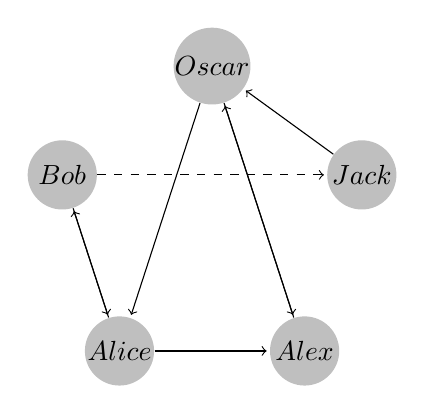
\begin{tikzpicture}[shorten >=1pt,->]
                        \tikzstyle{vertex}=[circle,fill=black!25,minimum size=25pt,inner sep=0pt]

                        \foreach \name/\angle/\text in {P-1/234/Alice, P-2/162/Bob,
                                  P-3/90/Oscar, P-4/18/Jack, P-5/-54/Alex}
                                \node[vertex,xshift=6cm,yshift=.5cm] (\name) at (\angle:2cm) {$\text$};

                        \draw (P-1) -- (P-5);
                        \draw[dashed,->] (P-2) -- (P-4);
                        \draw (P-4) -- (P-3);
                        \draw (P-3) -- (P-1);
                        \draw (P-1) -- (P-2);
                        \draw (P-2) -- (P-1);
                        \draw (P-3) -- (P-5);
                        \draw (P-5) -- (P-3);

                \end{tikzpicture}
                \caption{Communities of trust: Jack introduces Oscar to Bob's public-key certificate before Bob receives it.}
                \label{fig:web-of-trust}
        \end{center}
\end{figure}

\end{frame}

\begin{frame}{PGP}

	PGP inclut un certificat à clefs publiques et une chaîne de confiance(un \textbf{introducer}).\\
	\hfill \\
	Les niveaux de confiance pour un certificat sont :
	\begin{description}
		\item [Undefined] : on ne peut pas dire si la cle publique est valide ou pas
		\item [Marginal] : la clef publique \textbf{peut} être valide, mais on ne peut pas en être sûr
		\item [Complete] : on est sûr que la clef publique est valide
	\end{description}
	

\end{frame}

\begin{frame}{PGP}

	Les niveaux de confiance pour une chaîne de confiance (\textbf{introducer}) sont :
	\begin{description}
		\item [Full] : on peut faire totalement confiance à la clef publique pour introduire une nouvelle clef publique 
		\item [Marginal] : la clef publique \textbf{peut} introduire une nouvelle clef publique, mais on ne peut pas en être sûr
		\item [Untrustworthy] : on ne doit pas faire confiance à cette clef publique pour en introduire une nouvelle
	\end{description}

\end{frame}

\subsection{SKIP}

\begin{frame}{SKIP}

	\textbf{SKIP} (Simple Key-Management for Internet Protocol) implémente une chaîne d'authentificateurs de noeuds, où chaque noeud stocke ses informations dans une sorte de \textbf{directory service}\footnote{annuaire}.\\
	\hfill\\
	Etant donné que SKIP ne supporte pas la translation d'adresse (NAT par exemple), ce système est inutile.

\end{frame}

\section{Les systèmes en cours de développement}

\begin{frame}{Les systèmes en cours de développement}

	\begin{description}
		\item [DANE] (DNS-Based Authentication of Named Entities)
		\item [Sovereign keys] Les clefs souveraines par l'EFF\footnote{Electric Frontier Foundation}
		\item [CATA] (Certificate Authority Transparency and Auditability)
	\end{description}

\end{frame}

\subsection{DANE}

\begin{frame}{DANE}

	Ce système est arrivé avec une simple question : \textit{Pourquoi utiliser une nouvelle infrastructure de confiance alors que nous utilisons déjà DNS pour résoudre les noms de domaine ?}\\
	\hfill\\
	DANE utilise un nouveau champ dans la requête DNS\footnote{Sécurisé avec DNSEC} : le champ \textbf{TLSA}.
\begin{center}
\texttt{\_443.\_tcp.www.example.com. IN TLSA (\\
	~~~~~0 0 1 d2abde240d7cd3ee6b4b28c54df0\&34b9\\
	~~~~~7983a1d16e8a410e4561cb106618e971 )}
\end{center}

\end{frame}

\begin{frame}{DANE}

	\begin{figure}
		\centering
		\includegraphics[scale=0.35]{./../danereq.png}
		\caption{Fonctionnement de DANE}
	\end{figure}

\end{frame}

\subsection{Sovereign keys}

\begin{frame}{Sovereign keys}

	Le système de clefs souveraines s'appuie sur des \textbf{timeline servers}, sui seront en nombre restreint\footnote{Environ une vingtaine tout au plus}, gérant une liste publique dans laquelle on ne peut que faire des ajouts.\\
	
	Des clefs souveraines sont un couple de clefs cryptographiques où la clef publique est associée à un nom de domaine. Cette association est enregistrée dans les \textbf{timeline servers} cités précédemment.\\
	\hfill\\
	Cycle de vie des clefs souverraines :
	\begin{enumerate}
		\item Génération de la pair de clefs 
		\item Preuve de contrôle du domaine concerné (en utilisant PKI ou DANE)
		\item Ajout de la clef publique associée au nom de domaine dans les timeline servers
	\end{enumerate}
	
\end{frame}

\subsection{CATA}

\begin{frame}{CATA}

	Ce système se résume en une liste publique de certificats. Ainsi, chaque administrateur peut vérifier qu'il n'y a pas de fraude.\\
	Ceci dit, beaucoup de questions restent à résoudre :
	\begin{itemize}
		\item Qui doit gérer ces listes ?
		\item Combien de listes doivent être créées ?
		\item Comment la révocation doit fonctionner ?
		\item Qu'arrive-t-il si un certificat n'est plus disponible ?
	\end{itemize}
	
\end{frame}

\begin{frame}{Questions}
\begin{center}
	Avez-vous des questions ?
\end{center}


\end{frame}

\end{document}
